\subsection{Абсолютно неупругое соударение двух частиц.}
\textbf{Соударение (удар, столкновение)} — сильное кратковременное взаимодействие тел. Если нет силы реакции и внешние силы не успевают изменить импульс системы, можно применить \textit{Закон Сохранения Импульса}.

\begin{center}
	\begin{tikzpicture}[
		node distance=1cm and 0.5cm,
		box/.style={
			draw,
			rounded corners,
			fill=blue!20,
			minimum height=1cm,
			text width=2.5cm,
			align=center
		},
		arrow/.style={-Stealth, thick, blue!50!black}
		]
		\node[box, fill=red!30] (root) {\textbf{Удар}};
		\node[box, below left=of root] (left) {Абсолютно\\упругий};
		\node[box, below=of root] (middle) {Неупругий};
		\node[box, below right=of root] (right) {Абсолютно\\неупругий};
		\draw[arrow] (root) -- (left);
		\draw[arrow] (root) -- (middle);
		\draw[arrow] (root) -- (right);
	\end{tikzpicture}
\end{center}

\subsection{Абсолютно неупругий удар}

При абсолютно неупругом ударе тела соединяются и движутся как одно целое. Изменение кинетической энергии системы:

\begin{multline*}
	\Delta W_\text{кин} = \frac{m_1 + m_2}{2} v^2 - \left(\frac{m_1 v_1^2}{2} + \frac{m_2 v_2^2}{2}\right) = \\
	= \frac{(m_1 \vec{v}_1 + m_2 \vec{v}_2)^2}{2(m_1 + m_2)} - \frac{m_1 v_1^2}{2} - \frac{m_2 v_2^2}{2} = \\
	= \frac{m_1^2 v_1^2 + 2m_1m_2\vec{v}_1\vec{v}_2 + m_2^2v_2^2 - m_1(m_1 + m_2)v_1^2 - m_2(m_1 + m_2)v_2^2}{2(m_1 + m_2)} = \\
	= -\frac{m_1m_2(\vec{v_2} - \vec{v_1})^2}{2(m_1 + m_2)} = -\frac{m_{\text{пр}} v_{\text{отн}}^2}{2}
\end{multline*}

где $m_\text{пр} = \dfrac{m_1m_2}{m_1 + m_2}$ — приведённая масса.

Потерянная кинетическая энергия переходит в:
\begin{itemize}
	\item Тепловую энергию
	\item Энергию деформации
	\item Энергию вращения по теореме Кенинга: $W_\text{к} = \underbrace{W_\text{к}'}_\text{вращения} + \frac{m_1 + m_2}{2} v_c^2$
\end{itemize}

\begin{figure}[H]
	\centering
	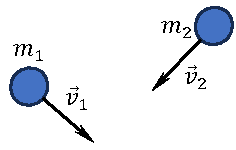
\includegraphics[width=0.5\linewidth]{image/Удар}
	\caption{Схема соударения двух тел}
	\label{fig:collision}
\end{figure}

\subsection{Абсолютно упругий удар}

Для сравнения приведём основные характеристики абсолютно упругого удара:

\begin{itemize}
	\item Сохранение кинетической энергии: $\frac{m_1 v_1^2}{2} + \frac{m_2 v_2^2}{2} = \frac{m_1 u_1^2}{2} + \frac{m_2 u_2^2}{2}$
	\item Сохранение импульса: $m_1\vec{v}_1 + m_2\vec{v}_2 = m_1\vec{u}_1 + m_2\vec{u}_2$
	\item Скорости после удара (1D случай):
	\[ u_1 = \frac{(m_1 - m_2)v_1 + 2m_2 v_2}{m_1 + m_2} \]
	\[ u_2 = \frac{(m_2 - m_1)v_2 + 2m_1 v_1}{m_1 + m_2} \]
\end{itemize}